% ----------------------------------------------------------
% CONFIGURAÇÃO DO DOCUMENTO
% ----------------------------------------------------------

\documentclass[
	% -- opções da classe memoir --
	12pt,				% tamanho da fonte
	openright,			% capítulos começam em pág ímpar (insere página vazia caso preciso)
	oneside,			% para impressão em verso e anverso. Oposto a oneside
	a4paper,			% tamanho do papel. 
	% -- opções da classe abntex2 --
	%chapter=TITLE,		% títulos de capítulos convertidos em letras maiúsculas
	%section=TITLE,		% títulos de seções convertidos em letras maiúsculas
	%subsection=TITLE,	% títulos de subseções convertidos em letras maiúsculas
	%subsubsection=TITLE,% títulos de subsubseções convertidos em letras maiúsculas
	% -- opções do pacote babel --
	english,			% idioma adicional para hifenização
	french,				% idioma adicional para hifenização
	spanish,			% idioma adicional para hifenização
	brazil				% o último idioma é o principal do documento
	]{abntex2}

% ----------------------------------------------------------
% IMPORTAÇÃO DE PACOTES
% ----------------------------------------------------------
\documentclass[
	% -- opções da classe memoir --
	12pt,				% tamanho da fonte
	openright,			% capítulos começam em pág ímpar (insere página vazia caso preciso)
	oneside,			% para impressão em verso e anverso. Oposto a oneside
	a4paper,			% tamanho do papel. 
	% -- opções da classe abntex2 --
	%chapter=TITLE,		% títulos de capítulos convertidos em letras maiúsculas
	%section=TITLE,		% títulos de seções convertidos em letras maiúsculas
	%subsection=TITLE,	% títulos de subseções convertidos em letras maiúsculas
	%subsubsection=TITLE,% títulos de subsubseções convertidos em letras maiúsculas
	% -- opções do pacote babel --
	english,			% idioma adicional para hifenização
	french,				% idioma adicional para hifenização
	spanish,			% idioma adicional para hifenização
	brazil				% o último idioma é o principal do documento
	]{abntex2}



% ---
% PACOTES BASICOS
% ---
\usepackage{lmodern}			% Usa a fonte Latin Modern			
\usepackage[T1]{fontenc}		% Selecao de codigos de fonte.
\usepackage[utf8]{inputenc}		% Codificacao do documento (conversão automática dos acentos)
\usepackage{lastpage}			% Usado pela Ficha catalográfica
\usepackage{indentfirst}		% Indenta o primeiro parágrafo de cada seção.
\usepackage{color}				% Controle das cores
\usepackage{graphicx}			% Inclusão de gráficos
\usepackage{microtype} 			% para melhorias de justificação

% ---
% PACOTES ADICIONAIS, USADOS APENAS NO ÂMBITO DO MODELO CANÔNICO DO abnteX2
% ---
\usepackage{lipsum}				% para geração de dummy text

% ---
% PACOTES DE CITAÇÕES
% ---
\usepackage[brazilian,hyperpageref]{backref}	 % Paginas com as citações na bibl
\usepackage[alf]{abntex2cite}	% Citações padrão ABNT

% ---
% PACOTES ADICIONADOS POR CEPHAS
% ---
\usepackage{float}
\usepackage{amssymb,amsmath}
\usepackage{pdfpages}
\usepackage{acronym}

% --- 
% CONFIGURAÇÕES DE PACOTES
% --- 

% Configurações do pacote backref
% Usado sem a opção hyperpageref de backref
\renewcommand{\backrefpagesname}{Citado na(s) página(s):~}
% Texto padrão antes do número das páginas
\renewcommand{\backref}{}
% Define os textos da citação
\renewcommand*{\backrefalt}[4]{
	\ifcase #1 %
		Nenhuma citação no texto.%
	\or
		Citado na página #2.%
	\else
		Citado #1 vezes nas páginas #2.%
	\fi}%
% ---

% ----------------------------------------------------------
% ELEMENTOS DA CAPA
% ----------------------------------------------------------
% ---
% Informações de dados para CAPA e FOLHA DE ROSTO
% ---
\titulo{Titulo do Seu Trabalho}
\autor{Aluno da Silva}
\local{Cidade-Estado}
\data{ano}
\orientador{titulo e nome do seu orientador}
\coorientador{titulo e nome do seu coorientador}
\instituicao{%
  Universidade Federal do Rio Grande do Norte -- UFRN
  \par
  Instituto Metrópole Digital -- IMD
  \par
  Programa de Pós-Graduação em Engenharia de Software -- PPgSW}
\tipotrabalho{Dissertação (Mestrado)}
% O preambulo deve conter o tipo do trabalho, o objetivo, 
% o nome da instituição e a área de concentração 
\preambulo{Dissertação de Mestrado  apresentada ao Programa de Pós-graduação em Engenharia de Software da Universidade Federal do Rio Grande do Norte como requisito para a obtenção do grau de Mestre em Engenharia de Software.}
% ---
% ----------------------------------------------------------
% APARENCIA DO PDF FINAL 
% ----------------------------------------------------------
% Configurações de aparência do PDF final

% alterando o aspecto da cor azul
\definecolor{blue}{RGB}{41,5,195}

% informações do PDF
\makeatletter
\hypersetup{
     	%pagebackref=true,
		pdftitle={\@title}, 
		pdfauthor={\@author},
    	pdfsubject={\imprimirpreambulo},
	    pdfcreator={LaTeX with abnTeX2},
		pdfkeywords={abnt}{latex}{abntex}{abntex2}{trabalho acadêmico}, 
		colorlinks=true,       		% false: boxed links; true: colored links
    	linkcolor=blue,          	% color of internal links
    	citecolor=blue,        		% color of links to bibliography
    	filecolor=magenta,      		% color of file links
		urlcolor=blue,
		bookmarksdepth=4
}
\makeatother
% --- 

% --- 
% Adicionado para evitar warning de Uppercase
% --- 
\pdfstringdefDisableCommands{\let\uppercase\relax}

% --- 
% Espaçamentos entre linhas e parágrafos 
% --- 

% O tamanho do parágrafo é dado por:
\setlength{\parindent}{1.3cm}

% Controle do espaçamento entre um parágrafo e outro:
\setlength{\parskip}{0.2cm}  % tente também \onelineskip

% ---
% compila o indice
% ---
\makeindex
% ---


% ----------------------------------------------------------
% ----------------------------------------------------------
% Início do documento
% ----------------------------------------------------------
% ----------------------------------------------------------
\begin{document}

% Seleciona o idioma do documento (conforme pacotes do babel)
\selectlanguage{brazil}
% Retira espaço extra obsoleto entre as frases.
\frenchspacing 

% ----------------------------------------------------------
% ELEMENTOS PRÉ-TEXTUAIS
% ----------------------------------------------------------
\pretextual

% ----------------------------------------------------------
% CAPA
% ----------------------------------------------------------
% Mude para usar capa limpa ou customizada (Includes/Capa.tex)
\imprimircapa

% ----------------------------------------------------------
% FOLHA DE ROSTO
% ----------------------------------------------------------
% Folha de rosto (o * indica que haverá a ficha bibliográfica)
\imprimirfolhaderosto*

% ----------------------------------------------------------
% FICHA BIBLIOGRAFICA
% ----------------------------------------------------------
% ---
% Inserir a ficha bibliografica
% ---

% Após defender seu mestrado vc deve seguir os passos no sigaa para submissão da sua dissertação à UFRN. A biblioteca lhe enviará via Sigaa a ficha bibliográfica em PDF. Se tiver tudo certo, importe ela como foi feito abaixo.
%
\begin{fichacatalografica}
    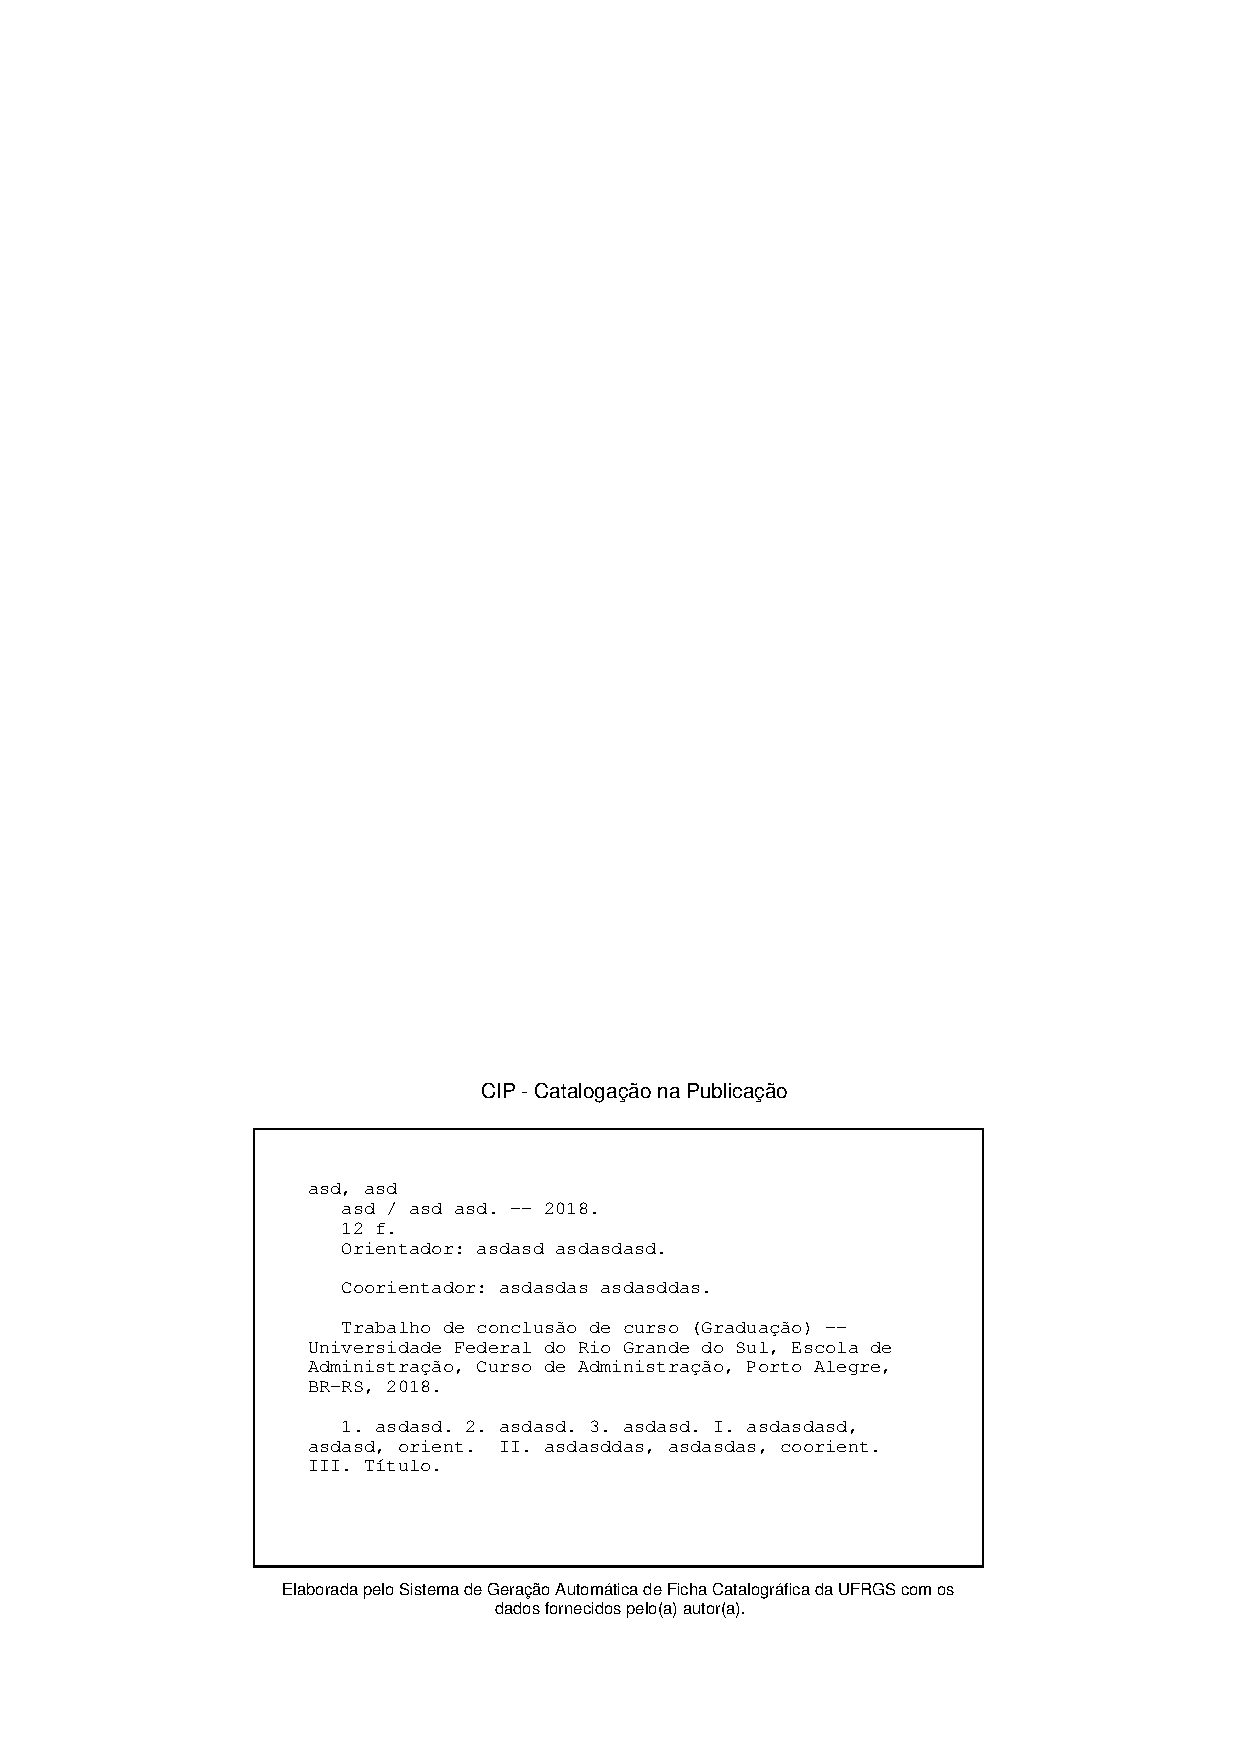
\includepdf[pages=-]{Includes/ficha.pdf}
\end{fichacatalografica}

% ----------------------------------------------------------
% ERRATA
% ----------------------------------------------------------
%\begin{errata}
%Elemento opcional da \citeonline[4.2.1.2]{NBR14724:2011}. Exemplo:

%Se não for usar, deixe o input no "main" comentado  

\vspace{\onelineskip}

FERRIGNO, C. R. A. \textbf{Tratamento de neoplasias ósseas apendiculares com
reimplantação de enxerto ósseo autólogo autoclavado associado ao plasma
rico em plaquetas}: estudo crítico na cirurgia de preservação de membro em
cães. 2011. 128 f. Tese (Livre-Docência) - Faculdade de Medicina Veterinária e
Zootecnia, Universidade de São Paulo, São Paulo, 2011.

\begin{table}[htb]
\center
\footnotesize
\begin{tabular}{|p{1.4cm}|p{1cm}|p{3cm}|p{3cm}|}
  \hline
   \textbf{Folha} & \textbf{Linha}  & \textbf{Onde se lê}  & \textbf{Leia-se}  \\
    \hline
    1 & 10 & auto-conclavo & autoconclavo\\
   \hline
\end{tabular}
\end{table}

\end{errata}
% ---

% ----------------------------------------------------------
% FOLHA DE APROVACAO
% ----------------------------------------------------------
% Folha de aprovação
\begin{folhadeaprovacao}
	%\setlength{\ABNTsignthickness}{0.4pt}
	%\setlength{\ABNTsignwidth}{10cm}
	
	% Informações gerais acerca do trabalho 
	% (nome do autor, título, instituição à qual é submetido e natureza)
	\noindent 
	Dissertação de Mestrado sob o título \textit{Título do Trabalho} apresentada por \textbf{aluno da Silva} e aceita pelo Programa de Pós-graduação em Engenharia de Software da Universidade Federal do Rio Grande do Norte, sendo aprovada por todos os membros da banca examinadora abaixo especificada:
		
	% Membros da banca examinadora e respectivas filiações
	\assinatura
	{
		Título e nome do professor  			                  \\
		{\small Presidente}											          \smallskip\\ 
		{\footnotesize
			IMD -- Instituto Metrópole Digital		   \\ %apenas um exemplo
		  	UFRN -- Universidade Federal do Rio Grande do Norte %apenas um exemplo
		}
   }
      
   \assinatura
	{
		Título e nome do professor  			                  \\
		{\small Examinador}											          \smallskip\\ 
		{\footnotesize
			SIGLA -- Institutição		   \\
		  	SIGLA -- Institutição
		}
   }   
   
   \assinatura
	{
		Título e nome do professor  			                  \\
		{\small Examinador}											          \smallskip\\ 
	    {\footnotesize
			SIGLA -- Institutição		   \\
		  	SIGLA -- Institutição
		}
	}
	
    \assinatura
	{
		Título e nome do professor  			                  \\
		{\small Examinador}											          \smallskip\\ 
		{\footnotesize
			SIGLA -- Institutição		   \\
		  	SIGLA -- Institutição
		}
	}
        
	\vfill
	
	\begin{center}
		Cidade-Estado, 01 de janeiro de 1915.
	\end{center}
\end{folhadeaprovacao}


\begin{folhadeaprovacao}

  \begin{center}
    {\ABNTEXchapterfont\large\imprimirautor}

    \vspace*{\fill}\vspace*{\fill}
    \begin{center}
      \ABNTEXchapterfont\bfseries\Large\imprimirtitulo
    \end{center}
    \vspace*{\fill}
    
    \hspace{.45\textwidth}
    \begin{minipage}{.5\textwidth}
        \imprimirpreambulo
    \end{minipage}%
    \vspace*{\fill}
   \end{center}
        
   Trabalho aprovado. \imprimirlocal, 01 de janeiro de 1915:

   \assinatura{\textbf{\imprimirorientador} \\ Orientador} 
   \assinatura{\textbf{título e nome do professor} \\ Examinador}
   \assinatura{\textbf{título e nome do professor} \\ Examinador}
   \assinatura{\textbf{título e nome do professor} \\ Examinador}
   %\assinatura{\textbf{Professor} \\ Convidado 4}
      
   \begin{center}
    \vspace*{0.5cm}
    {\large\imprimirlocal}
    \par
    {\large\imprimirdata}
    \vspace*{1cm}
  \end{center}
  
\end{folhadeaprovacao}


% ----------------------------------------------------------
% DEDICATORIA
% ----------------------------------------------------------
% Dedicatória

\chapter*{}
\vspace{15cm}
\begin{flushright}
	Texto de dedicatória.
\end{flushright}


% ----------------------------------------------------------
% AGRADECIMENTOS
% ----------------------------------------------------------
% Agradecimentos
\chapter*{Agradecimentos}

Agradeça a quem você desejar e da forma que você desejar. Este espaço pertence ao aluno e deve ter sua livre expressão de gratidão a quem desejar.

% ----------------------------------------------------------
% EPIGRAFE
% ----------------------------------------------------------
% Epígrafe (citação seguida de indicação de autoria)

\chapter*{}
\vspace{15cm}
\begin{flushright}
	\textit
	{
		Frase/texto que deseja citar
	}\medskip\\ 
	Autor.
\end{flushright}

% ----------------------------------------------------------
% RESUMO
% ----------------------------------------------------------
\chapter*{}
% Resumo em língua vernácula
\begin{center}
	{\Large{\textbf{Título do trabalho}}}
\end{center}

\vspace{1cm}

\begin{flushright}
	Autor: Aluno da Silva\\
	Orientador: Título e nome do Professor
\end{flushright}

\vspace{1cm}

\begin{center}
	\Large{\textsc{\textbf{Resumo}}}
\end{center}

\noindent 
resumo do trabalho em português.


\noindent\textit{Palavras-chave}: palavra\_1; palavra\_2; palavra\_3.






% ----------------------------------------------------------
% RESUMO
% ----------------------------------------------------------
\chapter*{}

% Resumo em língua estrangeira (em inglês Abstract, em espanhol Resumen, em francês Résumé)
\begin{center}
	{\Large{\textbf{Research Title in English}}}
\end{center}

\vspace{1cm}

\begin{flushright}
	Author: Aluno da Silva\\
	Supervisor: Título e nome do seu orientador
\end{flushright}

\vspace{1cm}

\begin{center}
	\Large{\textsc{\textbf{Abstract}}}
\end{center}

\noindent Research abstract fully in English.

\noindent\textit{Keyword\_s}: Word\_1; Word2; Word\_n.

% ----------------------------------------------------------
% LISTA DE ILUSTRACOES
% ----------------------------------------------------------
\chapter*{}
% ---
% inserir lista de ilustrações
% ---
\pdfbookmark[0]{\listfigurename}{lof}
\listoffigures*
\cleardoublepage
% ---

% ----------------------------------------------------------
% LISTA DE TABELAS
% ----------------------------------------------------------
% ---
% inserir lista de tabelas
% ---
\pdfbookmark[0]{\listtablename}{lot}
\listoftables*
\cleardoublepage
% ---

% ----------------------------------------------------------
% LISTA DE ABREVIATURAS E SIGLAS
% ----------------------------------------------------------
\chapter*{Lista de Abreviaturas}

\begin{acronym}

\acro{API}{\textit{Application Programming Interface}}      %exemplo
\acro{APIs}{\textit{Application Programming Interfaces}}    %exemplo
\acro{BTI}{Bacharelado em Tecnologia da Informação}         %exemplo

\end{acronym}

% ----------------------------------------------------------
% LISTA DE SIMBOLOS
% ----------------------------------------------------------
%não usei lista de símbolos, consulte o modelo canônico para mais detalhes

% ----------------------------------------------------------
% SUMARIO
% ----------------------------------------------------------
% ---
% inserir o sumario
% ---
\pdfbookmark[0]{\contentsname}{toc}
\tableofcontents*
\cleardoublepage
% ---

% ----------------------------------------------------------
% ----------------------------------------------------------
% ELEMENTOS TEXTUAIS
% ----------------------------------------------------------
% ----------------------------------------------------------
\textual

% ----------------------------------------------------------
% Introdução - CAPÍTULO 1
% ----------------------------------------------------------
\addcontentsline{toc}{chapter}{Capítulo 1}
% Introdução - vFinal 1.0 - 04-07-2018
\chapter{Titulo do Capítulo}
\label{cap:cap1}

Neste capítulo serão colocados textos de exemplo ou indicações para a contrução de uma Dissertação de mestrado em LateX. Uma parte será voltada à estrutura do documento e questões específicas relacionadas à ciência, e outra será dedicada a comandos simples e ``tricks" usados na construção do meu documento original.

Todo este template é apenas uma modularização e tentativa de simplificação do modelo disponível em \url{https://github.com/abntex/abntex2/wiki/Download}. Caso eu esqueça ou algum detalhe passe em branco, a dissertação inteira está disponível em \url{https://v1.overleaf.com/read/gpkgdnttndgf}.

Acredito também que este modelo sirva para outros programas, mas seu direcionamento principal, como já citado, é para o PPgSW - IMD - UFRN \cite{xiao_study_2011}. %citação incluída para nao deixar as referencias em branco

\section{Dicas para a dissertação e para a pesquisa}

\section{Sobre o \LaTeX}

% ----------------------------------------------------------
% CAPÍTULO 2
% ----------------------------------------------------------
\addcontentsline{toc}{chapter}{Capítulo 2}
% Capítulo 2 - vFinal 1.0 - 05/07/2018
\chapter{Conceitos Relacionados}
\label{cap:cap2}


% ----------------------------------------------------------
% PARTE
% ----------------------------------------------------------
%\part{Preparação da pesquisa}


% ----------------------------------------------------------
% Finaliza a parte (textual) no bookmark do PDF
% para que se inicie o bookmark na raiz
% e adiciona espaço de parte no Sumário
% ----------------------------------------------------------
\phantompart

% ----------------------------------------------------------
% ----------------------------------------------------------
% ELEMENTOS PÓS-TEXTUAIS
% ----------------------------------------------------------
% ----------------------------------------------------------
\postextual

% ----------------------------------------------------------
% Referências bibliográficas
% ----------------------------------------------------------
\bibliography{referencias}

% ----------------------------------------------------------
% Glossário
% ----------------------------------------------------------
%\glossary

% ----------------------------------------------------------
% Apêndices
% ----------------------------------------------------------
%% ---
% Inicia os apêndices
% ---
\begin{apendicesenv}

% Imprime uma página indicando o início dos apêndices
\partapendices
% ----------------------------------------------------------
\chapter{Título deste apendice}
% ----------------------------------------------------------

algum texto

% ----------------------------------------------------------
\chapter{título deste apendice}
% ----------------------------------------------------------
algum texto

\end{apendicesenv}

% ----------------------------------------------------------
% Anexos
% ----------------------------------------------------------
\begin{anexosenv}

% Imprime uma página indicando o início dos anexos
\partanexos

\chapter{Titulo deste anexo}
\label{anexo:anexo_mapa}
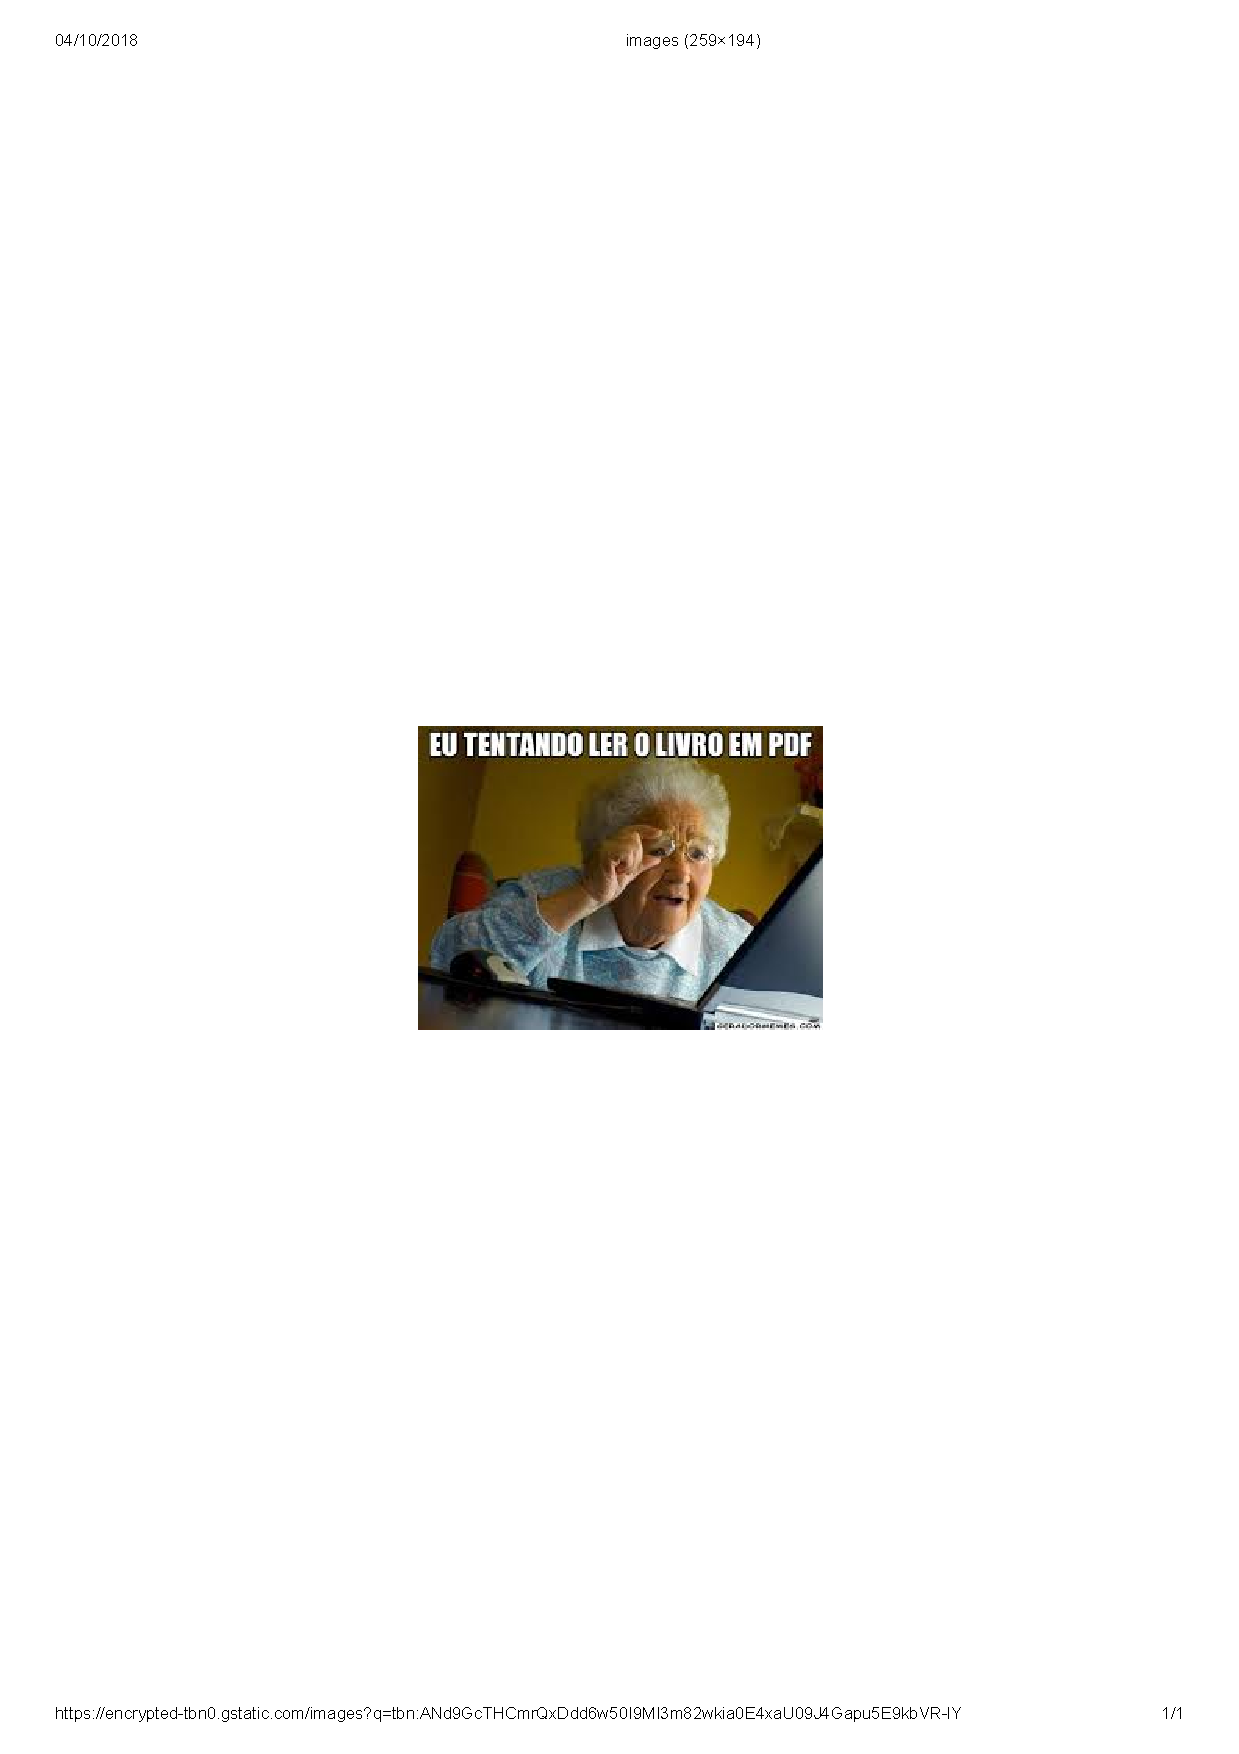
\includepdf[pages=-]{Anexos/exemplo.pdf}

\end{anexosenv}


%---------------------------------------------------------------------
% INDICE REMISSIVO
%---------------------------------------------------------------------

\phantompart
\printindex
%---------------------------------------------------------------------

\end{document}
